\documentclass[../main.tex]{subfiles}

\begin{document}


\subsubsection{Estimacion de días y costos}\label{sec:edc}

\begin{table}[H]
  \scriptsize
\centering
\begin{tabular}{|l|l|c|c|l|l|}
\hline
\rowcolor[HTML]{333333} 
{\color[HTML]{FFFFFF} \begin{tabular}[c]{@{}l@{}}Producto/\\ Referencia\end{tabular}} &
  {\color[HTML]{FFFFFF} Descripción} &
  \multicolumn{1}{l|}{\cellcolor[HTML]{333333}{\color[HTML]{FFFFFF} Cantidad}} &
  \multicolumn{1}{l|}{\cellcolor[HTML]{333333}{\color[HTML]{FFFFFF} Unidad}} &
  {\color[HTML]{FFFFFF} Valor Unitario} &
  {\color[HTML]{FFFFFF} Valor Total} \\ \hline
\rowcolor[HTML]{9AFF99} 
 &
  \begin{tabular}[c]{@{}l@{}}Subsistema área de\\ trabajo y  Salidas de datos\end{tabular} &
   &
   &
   &
  \$74,649.15 \\ \hline
 &
  \begin{tabular}[c]{@{}l@{}}Jack RJ45 Mini.com®\\  CAT 6a\end{tabular} &
  85 &
  unidad &
  \$250.00 &
  \$21,250.00 \\ \hline
 &
  \begin{tabular}[c]{@{}l@{}}Placa de pared de cuatro \\ Entradas (Tapa y caja)\end{tabular} &
  85 &
  unidad &
  \$599.99 &
  \$50,999.15 \\ \hline
 &
  Patchcord 6a &
  80 &
  unidad &
  \$30.00 &
  \$2,400.00 \\ \hline
\rowcolor[HTML]{9AFF99} 
 &
  Subsistema horizontal &
   &
   &
   &
  \$5,300.00 \\ \hline
 &
  Cable UTP de Datos Cat 6a &
  1 &
  305 {[}m{]} &
  \$5,300.00 &
  \$5,300.00 \\ \hline
\rowcolor[HTML]{9AFF99} 
 &
  \begin{tabular}[c]{@{}l@{}}Subsistema Gabinete de\\ Telecomunicaciones\end{tabular} &
   &
   &
   &
  \$15,200.00 \\ \hline
 &
  Cable UTP de Datos Cat 6a &
  3 &
  unidad &
  \$1,600.00 &
  \$4,800.00 \\ \hline
WMPHF2E &
  \begin{tabular}[c]{@{}l@{}}Organizador Horizontal\\ Frontal 2ur\end{tabular} &
  4 &
  unidad &
  \$900.00 &
  \$3,600.00 \\ \hline
WMPVF45E &
  \begin{tabular}[c]{@{}l@{}}Organizador Vertical \\ Frontal 2ur\end{tabular} &
  4 &
  unidad &
  \$1,700.00 &
  \$6,800.00 \\ \hline
\rowcolor[HTML]{9AFF99} 
 &
  Fibra Óptica &
   &
   &
   &
  \$57,767.99 \\ \hline
 &
  \begin{tabular}[c]{@{}l@{}}Fibra Óptica 12 hilo 70 metros,\\  Multimodo 50/125μ\end{tabular} &
  70 &
  metro &
  \$450.00 &
  \$31,500.00 \\ \hline
FLCSMCXAQY &
  \begin{tabular}[c]{@{}l@{}}Conector Simplex pre-pulido lc\\ Opticam® multimodo 50/125\end{tabular} &
  24 &
  unidad &
  \$602.00 &
  \$14,448.00 \\ \hline
FAP12WBRDDLCZ &
  \begin{tabular}[c]{@{}l@{}}Panel de adaptadores de fibra LC 10 Gig\\  OM3/OM4 cargado con doce adaptadores\\  de fibra optica LC 10Gig duplex multimodo\end{tabular} &
  1 &
  unidad &
  \$5,000.00 &
  \$5,000.00 \\ \hline
FAP6WAQDLC &
  \begin{tabular}[c]{@{}l@{}}Panel de 6 Adaptadores de Fibra Óptica\\  LC 10Gig OM3/OM4 Dúplex Multimodo\end{tabular} &
  1 &
  unidad &
  \$1,750.00 &
  \$1,750.00 \\ \hline
FXE3-10M3Y &
  \begin{tabular}[c]{@{}l@{}}Jummper de Fibra Duplex  lc-lc \\ 50/125μm (om3/om4)\end{tabular} &
  1 &
  3 {[}m{]} &
  \$869.99 &
  \$869.99 \\ \hline
FHD-2UFCE &
  Distribuidor de fibra de 2U &
  1 &
  unidad &
  \$4,200.00 &
  \$4,200.00 \\ \hline
\rowcolor[HTML]{9AFF99} 
 &
  Equipos y Dispositivos &
   &
   &
   &
  \$208,497.00 \\ \hline
WAP581-B-K9 &
  Access Point Cisco &
  4 &
  unidad &
  \$5,700.00 &
  \$22,800.00 \\ \hline
WS-C2960X-48TS-L &
  Switch CISCO 48 puertos &
  2 &
  unidad &
  \$67,899.00 &
  \$135,798.00 \\ \hline
WS-C2960X-24S-L &
  Switch CISCO 24 puertos &
  1 &
  unidad &
  \$49,899.00 &
  \$49,899.00 \\ \hline
 &
   &
   &
  \multicolumn{1}{l|}{} &
   &
   \\ \hline
 &
   &
   &
  \multicolumn{1}{l|}{} &
  \cellcolor[HTML]{333333}{\color[HTML]{FFFFFF} Total} &
  \cellcolor[HTML]{333333}{\color[HTML]{FFFFFF} \$361,414.14} \\ \hline
\end{tabular}\label{cot}
\caption{Cotización, Productos}
\end{table}


\begin{figure}[H]
  \centering
  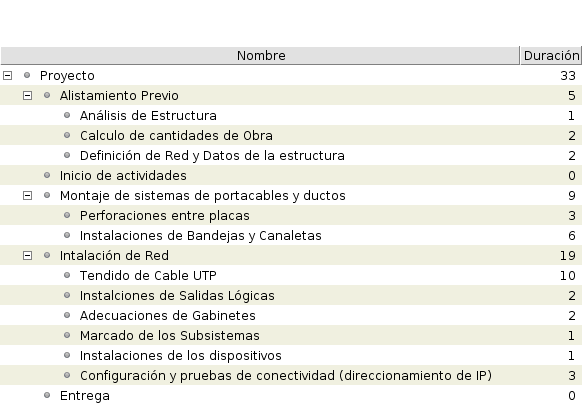
\includegraphics[scale=0.6]{actividades}
  \caption{Cronograma}\label{fig:crono}
  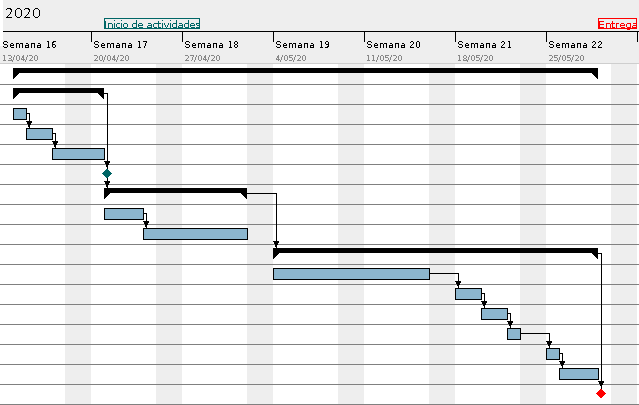
\includegraphics[scale=0.54]{actividades_2}
  \caption{Cronograma Gráfico}\label{fig:cronog}
\end{figure}

Como vemos en la figura \ref{fig:crono} la instalación de la red para el
segundo piso consta de \textbf{61} días laborables añadiendo un costo
de mano de obra de $\$300,000.00$MXN.\@

Por lo tanto, el costo  para instalar la red en el segundo
piso del \acrshort{igg}\@ es a un aproximado de $\$661,414.14$MXN --- SEISCIENTOS SESENTA Y
UN MIL CUATROCIENTOS CATORCE 14/100 MXN.\@ 
                                                         
\end{document}
